%\documentclass[onecolumn]{IEEEtranTIE}
\documentclass[journal]{IEEEtranTIE}
\usepackage{graphicx}
%\usepackage{cite}
\usepackage{picinpar}
\usepackage{amsmath}
%\usepackage{url}
\usepackage{flushend}
\usepackage{colortbl}
\usepackage{soul}
\usepackage{multirow}
\usepackage{pifont}
\usepackage{color}
\usepackage{alltt}
\usepackage[hidelinks]{hyperref}
\usepackage{enumerate}
\usepackage{siunitx}
\usepackage{breakurl}
\usepackage{epstopdf}
\usepackage{pbox}
\usepackage[portuguese]{babel}
\usepackage{float}
\usepackage[utf8]{inputenc}
\usepackage{textcomp}
\usepackage{mathrsfs}

\begin{document}
\title{PalmPlant: Kit Didático de Controle}
\author{
	\vskip 1em
    	{
        	\textsc{Piaia, Guilherme} \\
            \textsc{\textbf{Professor}: Rodrigo Iván Goytia Mejía} \\
			\normalsize Universidade do Vale do Rio dos Sinos \\
        }
	   }

\maketitle

\begin{abstract}
No relatório apresentado descrever-se-a o desenvolvimento de um kit didático de controle, baseado em um sistema embarcado e um servidor web, onde pode ser inserido o modelo desejado, e o kit se comportará conforme o modelo inserido, criando-se assim, um irmão gêmeo.
\end{abstract}

\markboth{Relatório de Modelagem de Sistemas - Mestrado Pofissional em Engenharia Elétrica $\quad\diamond\quad$ Julho de 2019}{}
	\maketitle

\definecolor{limegreen}{rgb}{0.2, 0.8, 0.2}
\definecolor{forestgreen}{rgb}{0.13, 0.55, 0.13}
\definecolor{greenhtml}{rgb}{0.0, 0.5, 0.0}

%%%%%%%%%%%%%%%%%%%%%%%%%%%%%%%%%%%%%%%%%%%%%%%%%%%%%%%%%%%%%%%%%%%%%%%%%%%%%%%

\section{Introdução}

\IEEEPARstart{O} modelo escolhido foi um satélite simplificado, ou seja, um cubo de aço inoxidável com 4 rodas de reação, sendo dois pares opostos interligados por um eixo.

O satélite cúbico possui \SI{300}{\mm} de lados, e as rodas possuem \SI{75}{\mm} de raio e \SI{30}{\mm} de espessura
O satélite pode ser visto na imagem da sequência:

\begin{figure}[H]
	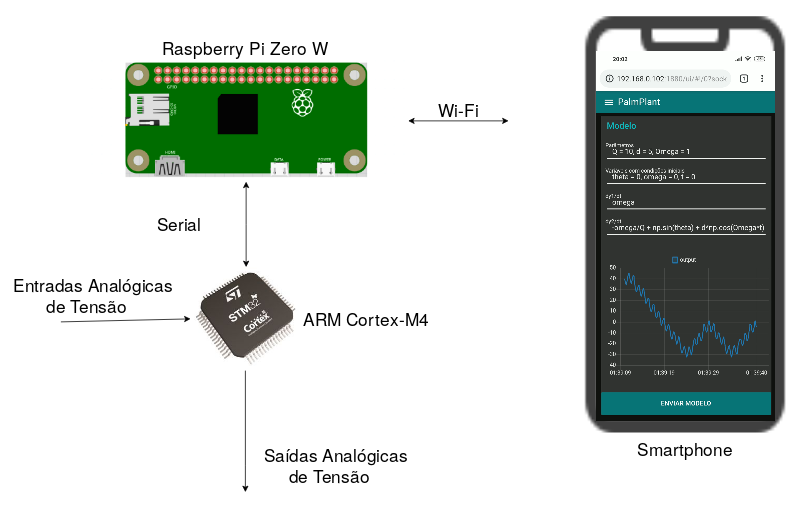
\includegraphics[width=\linewidth]{img/diagrama.png}
    \caption{Diagrama do Kit. Fonte: elaborado pelo autor}
    \label{fig:real}
\end{figure}


\begin{figure}[H]
	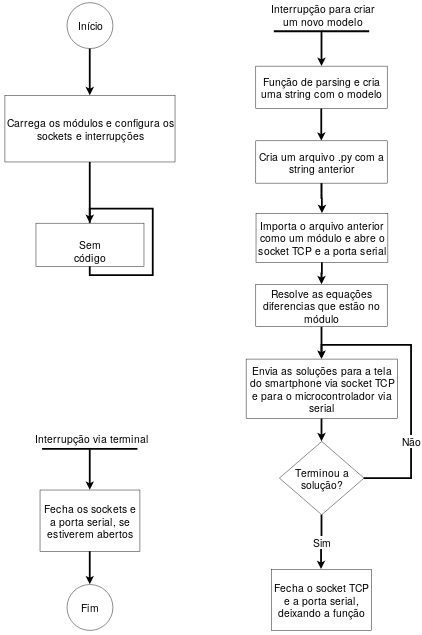
\includegraphics[width=\linewidth]{img/software.png}
    \caption{Diagrama do Kit. Fonte: elaborado pelo autor}
    \label{fig:real}
\end{figure}

\begin{figure}[H]
	\centering
	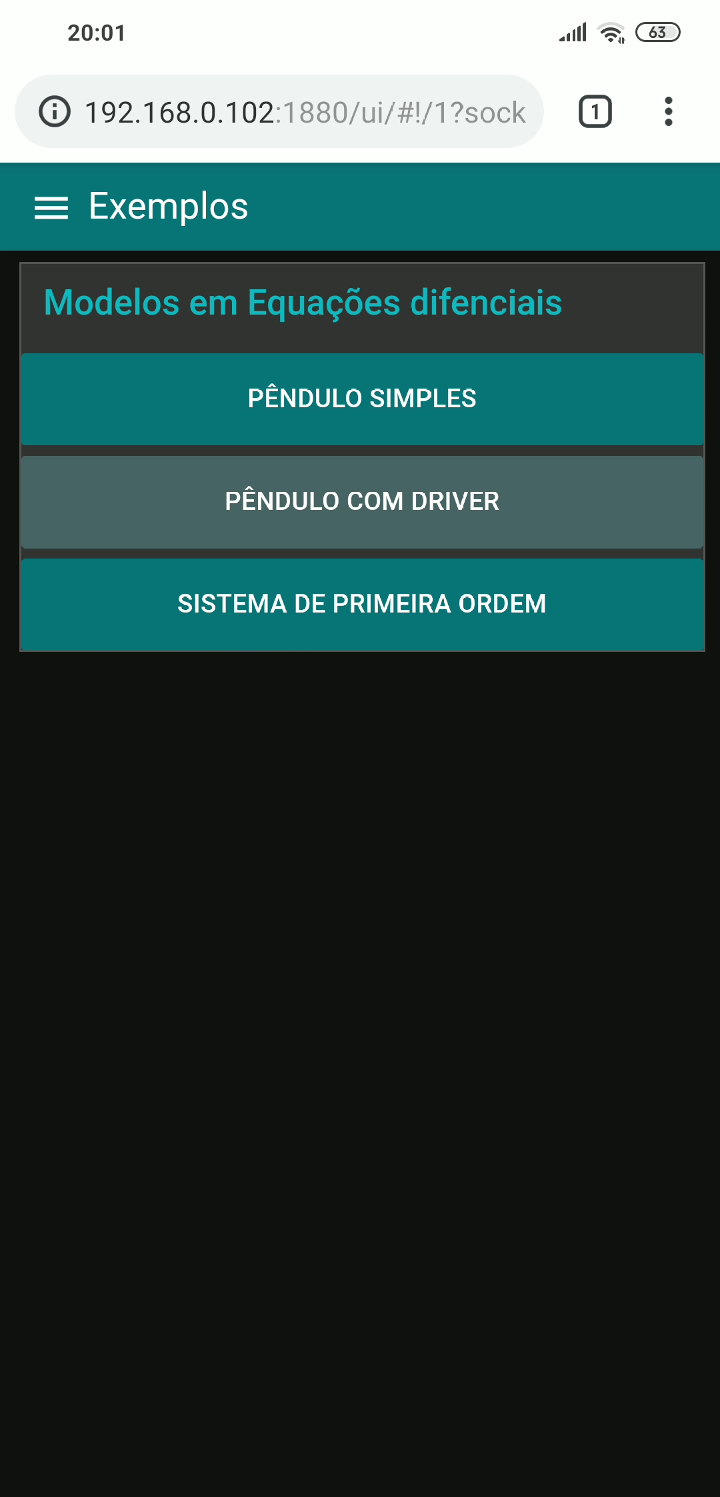
\includegraphics[width=4.1cm]{img/examples.png}
    \caption{Tela com exemplos de modelos. Fonte: elaborado pelo autor}
    \label{fig:examples}
\end{figure}


\begin{figure}[H]
	\centering
	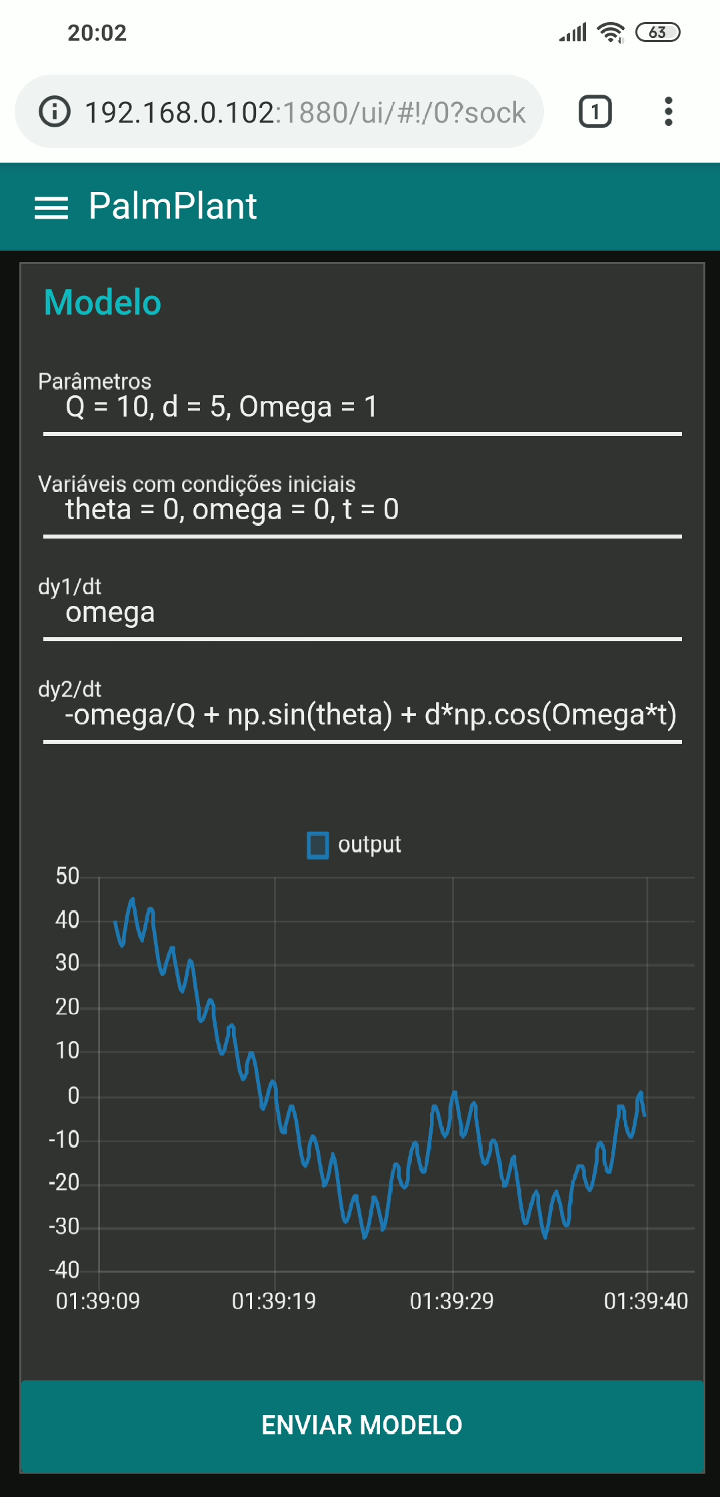
\includegraphics[width=4.1cm]{img/running.png}
    \caption{Tela de edição dos modelos e visualização da solução. Fonte: elaborado pelo autor}
    \label{fig:running}
\end{figure}


\begin{figure}[H]
	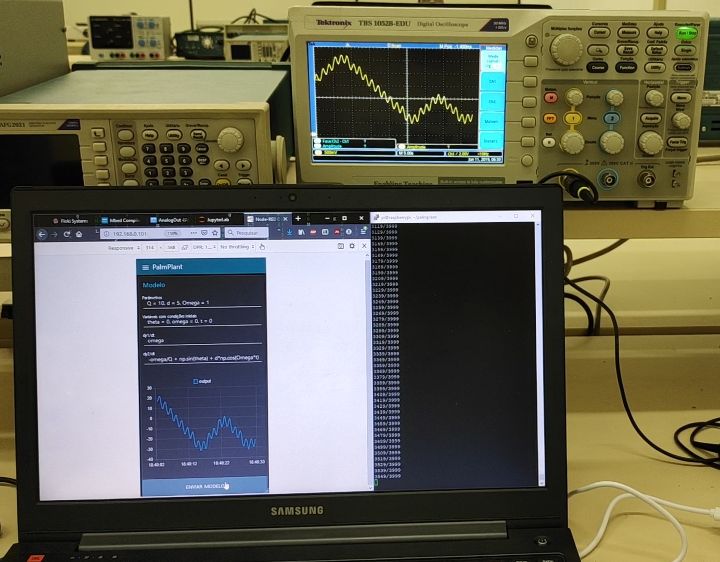
\includegraphics[width=\linewidth]{img/real_running.png}
    \caption{Funcionamento da saída analógica de tensão. Fonte: elaborado pelo autor}
    \label{fig:real}
\end{figure}


 \begin{enumerate}[1.]
   	 	\item O satélite é um cubo sólido com densidade homogênea;
   	 	\item As rodas também são sólidas e homogêneas;
   	 	\item O satélite se encontra estático no espaço sideral, não sofrendo nenhuma força significante;
   		\item A temperatura em que ele se encontra não prejudica o normal funcionamento
\end{enumerate}

%%%%%%%%%%%%%%%%%%%%%%%%%%%%%%%%%%%%%%%%%%%%%%%%%%%%%%%%%%%%%%%%%%%%%%%%%%%%%

\section{Desenvolvimento}


%%%%%%%%%%%%%%%%%%%%%%%%%%%%%%%%%%%%%%%%%%%%%%%%%%%%%%%%%%%%%%%%%%%%%%%%%%%%%

\section{Resultados}


%%%%%%%%%%%%%%%%%%%%%%%%%%%%%%%%%%%%%%%%%%%%%%%%%%%%%%%%%%%%%%%%%%%%%%%%%%%%%

\section{Conclusão}


%%%%%%%%%%%%%%%%%%%%%%%%%%%%%%%%%%%%%%%%%%%%%%%%%%%%%%%%%%%%%%%%%%%%%%%%%%%%%

 \section{Bibliografia}
[1] Nise, Norman. \textbf{Engenharia de Sistemas de Controle}, 5. ed. editora LTC, 2011

[2] Ogata, Katsuhiko. \textbf{Engenharia de Controle Moderno}. 5. ed. editora Prentice Hall Brasil, 2010
\end{document}
